\problemname{Fake Snowflake}

\noindent
Alexander is a climate change denier and wants to prove to Joshua that the Earth is not getting warmer at all.
Alexander argues that it has already snowed several times in November,
which suggests that the temperature is dropping. Joshua, who mostly stays indoors,
hasn't noticed any snow.
Therefore, Alexander has been running around taking pictures of a lot of particles in the air,
hoping to show photographic evidence to Joshua.
Now, he has finally taken a picture he is quite satisfied with,
but he needs to make some changes before showing the image.

Joshua, who loves fractals and unnecessarily complicated things,
has specific ideas about how a snowflake should look.
An image consists of $N \times N$ pixels, where $N$ is an odd number,
and each pixel is either white or black.
The snowflake is made up of the white pixels in the image.
According to Joshua, the image represents a snowflake if the following criteria are met:

\begin{itemize}
  \item The center pixel is white.
  \item If you rotate the image clockwise 90 degrees, it looks the same.
  \item If you mirror the image along the vertical centerline, it looks the same.
  \item There are no $2 \times 2$ squares consisting entirely of white pixels.
  \item The set of white pixels is contiguous \emph{without diagonal steps}.
    This means that if you start with a pen on any white pixel, you can
    access every other white pixel without lifting the pen and without
    drawing on black pixels.
    The pen can go up, down, left and right, \emph{but not} diagonally.
  \item The set of black pixels is contiguous \emph{with diagonal steps}.
    This means that if you start with a pen on any black pixel, you can
    access every other black pixel without lifting the pen and without
    drawing on white pixels.
    The pen can go up, down, left, right, \emph{and} diagonally.
  \item There are no hooks in the snowflake.
  Let $\text{pixel}_\text{up}$, $\text{pixel}_\text{right}$, $\text{pixel}_\text{down}$,
  and $\text{pixel}_\text{left}$ be the adjacent pixels to a white pixel.
  A hook occurs if exactly two of these adjacent pixels are also white,
  and they are not on opposite sides of the pixel.
  For example, if $\text{pixel}_\text{up}$ and $\text{pixel}_\text{right}$ are white while
  $\text{pixel}_\text{down}$ and $\text{pixel}_\text{left}$ are black, a hook is formed,
  but if $\text{pixel}_\text{up}$ and $\text{pixel}_\text{down}$ are white
  and $\text{pixel}_\text{right}$ and $\text{pixel}_\text{left}$ are black, a hook is not formed.

\end{itemize}

\begin{figure}[h]
    \centering
    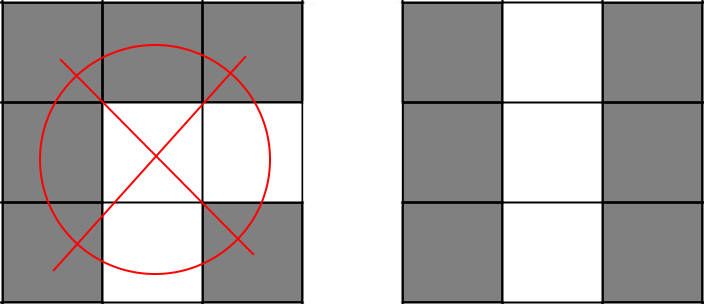
\includegraphics[scale=0.2]{crook_example.png}
    \caption{Two $3 \times 3$ images. The three pixels on the left form a hook, which is not allowed. The three pixels on the right do not form a hook.}
    \label{fig:enter-label}
\end{figure}

\begin{centering}
    \begin{figure}[h]
        \centering
        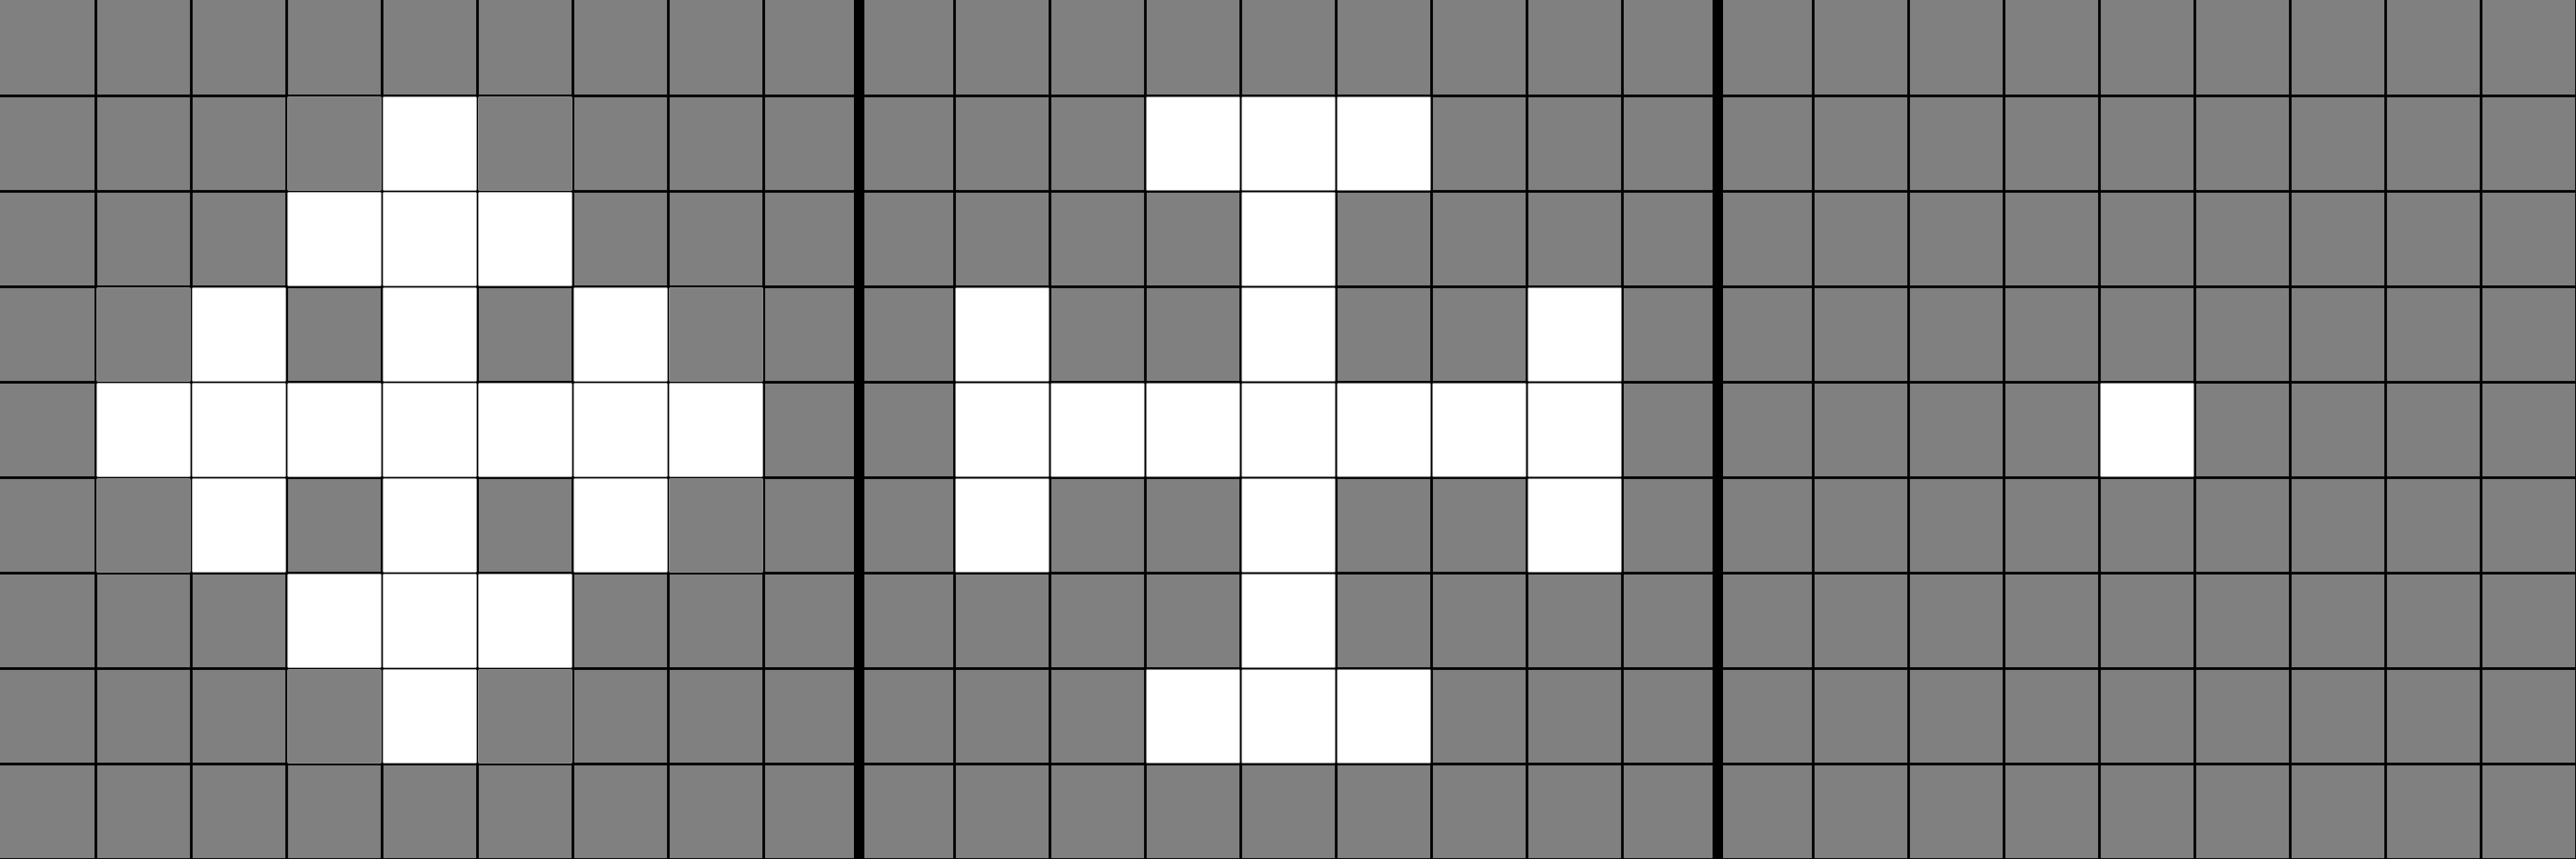
\includegraphics[scale=0.1]{all_valid_examples.png}
        \caption{Three examples of $9 \times 9$ images depicting snowflakes.}
        \label{fig:enter-label}
    \end{figure}
\end{centering}

\begin{centering}
    \begin{figure}[h]
        \centering
        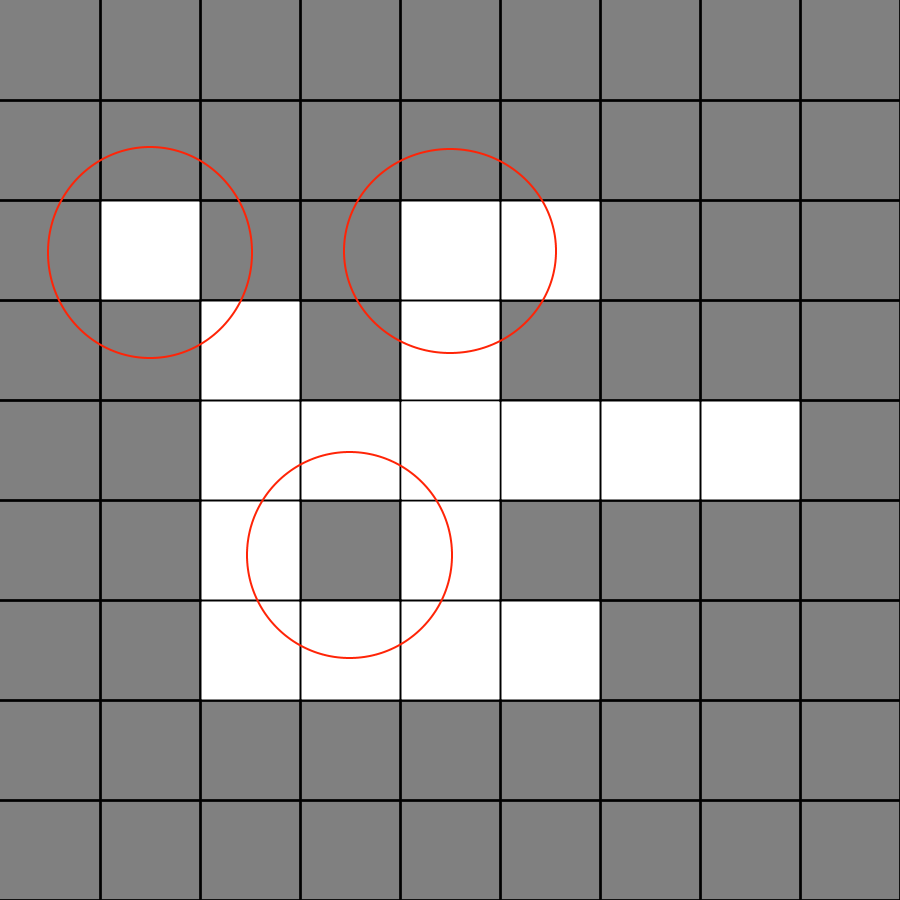
\includegraphics[scale=0.1]{invalid_example.png}
        \caption{A very inaccurate snowflake. Of the three circled pixels, one white pixel is not contiguous with the rest of the white pixels, one pixel forms a hook, and one black pixel is not contiguous with the rest of the black pixels. Additionally, the image does not satisfy any of the two symmetry requirements.}
        \label{fig:enter-label}
    \end{figure}
\end{centering}

\noindent
Alexander has downloaded an image editing program where he can change the color of pixels,
both from black to white and from white to black.
Since he's not very skilled at image editing, Alexander expects it to take him one minute
for each pixel he needs to change.
Alexander is a very busy man and wants to be as time-efficient as possible.
He now wants to know how quickly he can finish if he changes as few pixels as possible.

\section*{Input}

The first line of the input contains the odd integer $N$ ($7 \le N \le 15$), the number of pixels on each side of the square image.
Then there are $N$ lines of input, where the $i$-th line contains the $N$ numbers $p_{i,1}, p_{i,2}, ..., p_{i,N}$.
If the pixel at position ($i, j$) in the image is white, then $p_{i, j} = 1$, otherwise $p_{i, j} = 0$.
Position (1,1) corresponds to the pixel in the upper left corner.


\section*{Output}

Print an integer: the minimum number of minutes it takes for Alexander to make changes
to his image for Joshua to agree that the image represents a snowflake.

\section*{Scoring}

Your solution will be tested on a set of test case groups.
To score points for a group, you must pass all the test cases in that group.

\begin{tabular}{| l | l | p{12cm} |}
  \hline
  \textbf{Group} & \textbf{Points} & \textbf{Limits} \\ \hline
  $1$    & $20$       & $N=7$ \\ \hline
  $2$    & $20$       & $N=11$ \\ \hline
  $3$    & $60$       & $N=15$ \\ \hline
\end{tabular}
